\chapter{Phenomenological Studies of the Diphoton Process in Proton-Proton
  Scattering}%
\label{chap:pheno}

\begin{figure}[h!]
  \centering
  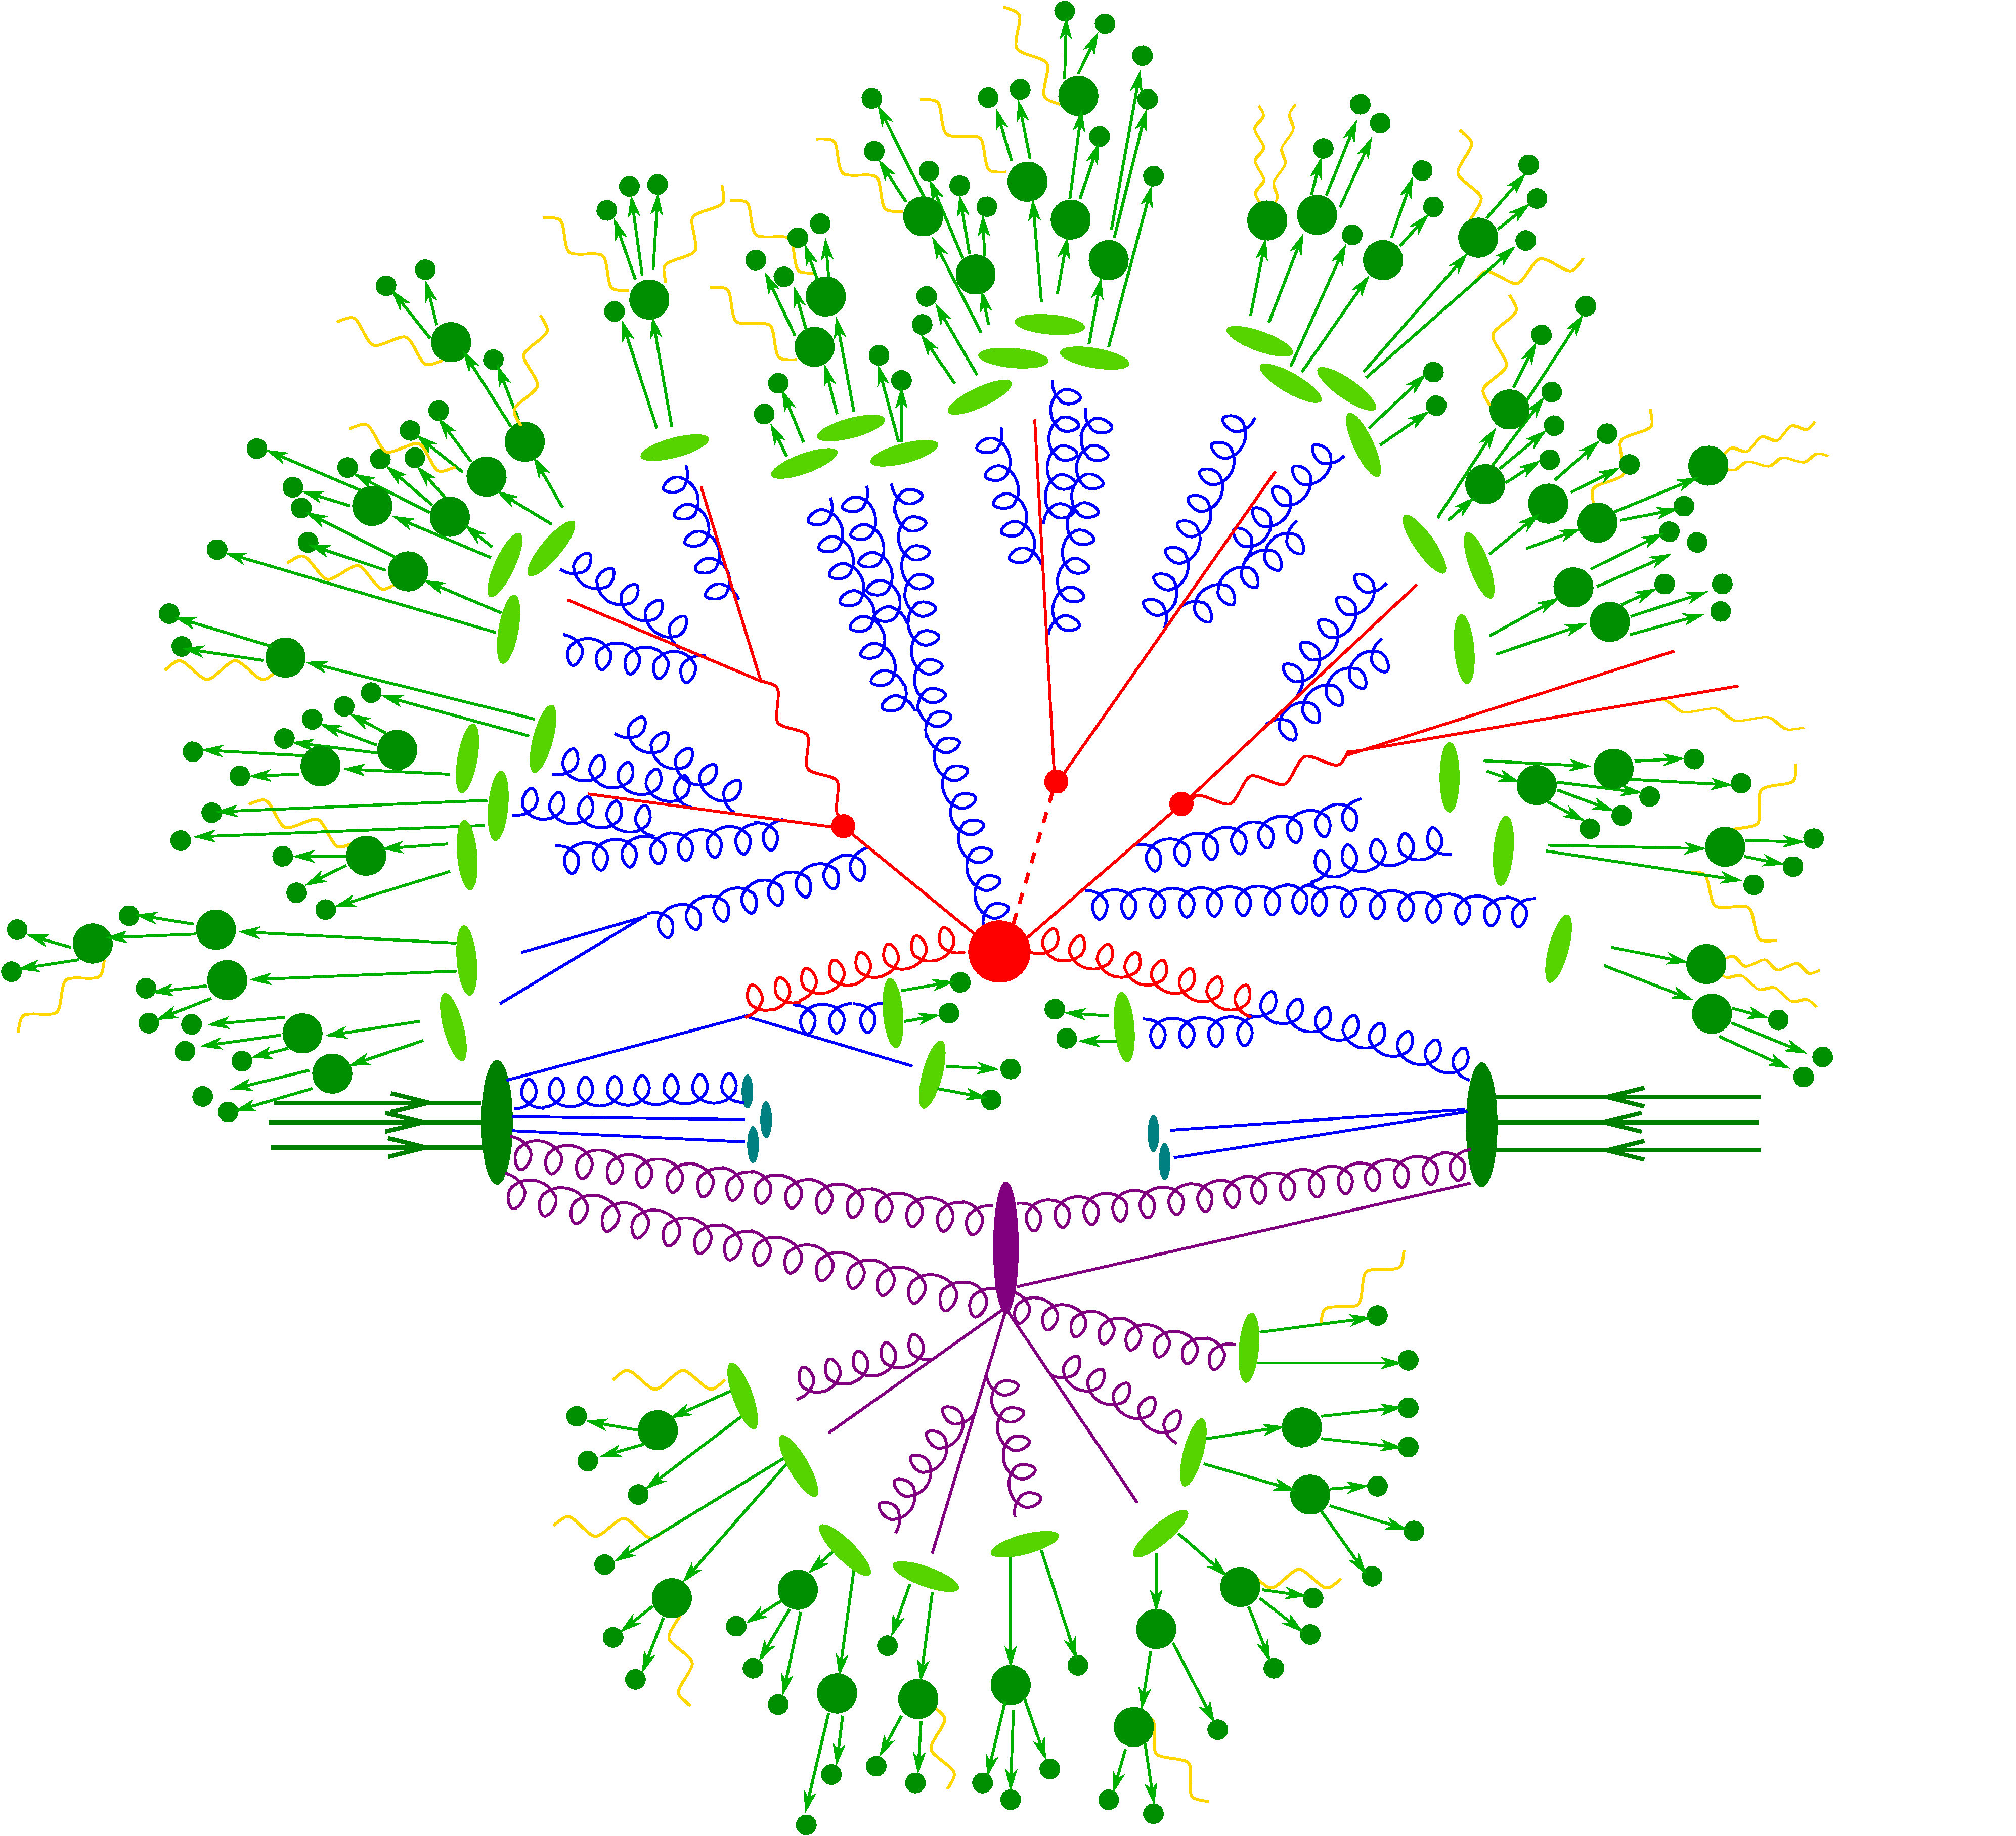
\includegraphics[width=.6\textwidth]{figs/event.pdf}
  \caption[The anatomy of a \(t\bar{t}h\) event.]{\label{fig:anatomy}
    The anatomy of a \(t\bar{t}h\) event. Taken
    from~\cite{Gleisberg:2008ta}. Described below.}
\end{figure}
%
In real proton scattering the hard process discussed in
\cref{chap:pdf} is only a part of the whole event. \Cref{fig:anatomy}
shows a pictorial representation of the plethora of processes taking
place around the hard event (red), marking distinct processes in the
event generator by different colors.  Partons do in general have some
intrinsic transverse momentum.  Scattered charges radiate in both QCD
and QED, both giving rise to shower-like cascades (blue, yellow) and
both can lead to additional transverse momentum of the initial state
partons. The remnants of the proton can radiate showers themselves,
scatter in more or less hard processes (Multiple Interactions, MI,
purple blob) and affect the hard process through color
correlation. Finally the partons from the showers recombine into
hadrons (hadronization, light green blobs) due to QCD
confinement. This last effect doesn't produce diphoton-relevant
background directly, but affects photon isolation. Those hadrons then
decay if they are unstable (dark green blobs), producing even more
final state particles. All of those processes have to be taken into
account to generate events that can be compared with experimental
data.~\cite{buckley:2011ge,Gleisberg:2008ta}

These effects can be calculated or modeled on an per-event base by
modern Monte Carlo event generators like \sherpa. But these
calculations and models are approximations in most cases. This is done
for the diphoton process in a gradual way described in
\cref{sec:setupan}. Histograms of observables are generated and
discussed in \cref{sec:disco}.

%%% Local Variables:
%%% mode: latex
%%% TeX-master: "../document"
%%% End:
